% REMEMBER TO SET LANGUAGE!
\documentclass[a4paper,10pt,english]{article}
\usepackage[utf8]{inputenc}
\usepackage{cite}
\usepackage{braket}
\usepackage{enumitem}

% Standard stuff
\usepackage{amsmath,amsthm, amssymb,graphicx,varioref,verbatim,amsfonts,geometry,esint,url,color}
% colors in text
\usepackage[usenames,dvipsnames,svgnames,table]{xcolor}
% Hyper refs
\usepackage[colorlinks]{hyperref}
\usepackage{float}
\usepackage{wrapfig}

\usepackage{tikz}
\usepackage[framemethod=tikz]{mdframed}
\usepackage{tikz-3dplot}
\usetikzlibrary{matrix,calc}

\usepackage{bm}

\usepackage[export]{adjustbox}

\usepackage{subfig}
\usepackage{algpseudocode}
\usepackage{algorithm}
\usepackage[makeroom]{cancel}
\usepackage{wasysym}

\usepackage{tcolorbox}
\tcbuselibrary{most}

%%%%%FOR THE enumitem PACKAGE
\setlist[enumerate]{label*=\arabic*.}
%%%%%

%%%%EXAMPLE ENVIRONMENT

\newtcolorbox
[auto counter,number within=section]{pabox}[2][]{
%
enhanced,colback=black!5!white, colframe=black, fuzzy shadow={0mm}{-4pt}{-0.5pt}{0.4mm}{black!60!white},
title=Example 
\thetcbcounter
: #2,#1}

\newcommand{\example}[2]{
\begin{pabox}[label={myautocounter}]{#1}
#2
\end{pabox}
}
%%%%%%%%%%%%%%%%%%%%%%

%%%% BOX EQUATION ENVIRONMENT

\newenvironment{boxequation}{
\begin{tcolorbox}[ams equation, enhanced, colback=black!50!green!10!white, colframe=black, fuzzy shadow={0mm}{-4pt}{-0.5pt}{0.4mm}{black!60!white}]}
{\end{tcolorbox}}
%%%%%%%%%%%%%%%%%%%%%%%%%%%%%

%%%% BOX QUOTE ENVIRONMENT

\newenvironment{boxquote}{
\begin{tcolorbox}[enhanced, colback=black!50!green!10!white, colframe=black, fuzzy shadow={0mm}{-4pt}{-0.5pt}{0.4mm}{black!60!white}]
\begin{center}}
{\end{center}\end{tcolorbox}}

%%%%%%%%%%%%%%%%%%%%%%%%%%

% Document formatting
\setlength{\parindent}{0mm}
\setlength{\parskip}{1.5mm}


%Color scheme for listings
\usepackage{textcomp}
\definecolor{listinggray}{gray}{0.9}
\definecolor{lbcolor}{rgb}{0.9,0.9,0.9}

\usepackage{listings}
\lstset{
	backgroundcolor=\color{lbcolor},
	tabsize=4,
	rulecolor=,
	language=python,
        basicstyle=\scriptsize,
        upquote=true,
        aboveskip={1.5\baselineskip},
        columns=fixed,
	numbers=left,
        showstringspaces=false,
        extendedchars=true,
        breaklines=true,
        prebreak = \raisebox{0ex}[0ex][0ex]{\ensuremath{\hookleftarrow}},
        frame=single,
        showtabs=false,
        showspaces=false,
        showstringspaces=false,
        identifierstyle=\ttfamily,
        keywordstyle=\color[rgb]{0,0,1},
        commentstyle=\color[rgb]{0.133,0.545,0.133},
        stringstyle=\color[rgb]{0.627,0.126,0.941}
        }
        
\DeclareMathOperator{\dist}{dist}
\newcommand{\distx}{\dist x}
        
\newcounter{subproject}
\renewcommand{\thesubproject}{\alph{subproject}}
\newenvironment{subproj}{
\begin{description}
\item[\refstepcounter{subproject}(\thesubproject)]
}{\end{description}}


\definecolor{ubuntu_terminal_background}{RGB}{48,10,36}

\lstdefinestyle{DOS}
{
    backgroundcolor=\color{ubuntu_terminal_background},
    basicstyle=\scriptsize\color{white}\ttfamily
}

\lstnewenvironment{terminal}[1]
  {%
   \mdframed[backgroundcolor = ubuntu_terminal_background, innertopmargin = -0.4cm, innerbottommargin = -0.1cm, hidealllines = true, innerleftmargin = 0.2cm, innerrightmargin = 0.2cm]%
   \lstset{
     backgroundcolor=\color{ubuntu_terminal_background}, keywords={},
     basicstyle=\scriptsize\color{white}\ttfamily, frame = none, numbers=none
   }%
  }
  {\endmdframed}


%%%%%%%%%%%%%%  VECTORS TO BOLD
\let\oldhat\hat
\renewcommand{\vec}[1]{\mathbf{#1}}
%%%%%%%%%%%%%%  

%%%%%%%%%%%%%% UNIT VECTOR 
\newcommand{\uveci}{{\bm{\hat{\textnormal{\bfseries\i}}}}}
\newcommand{\uvecj}{{\bm{\hat{\textnormal{\bfseries\j}}}}}
\DeclareRobustCommand{\uvec}[1]{{%
  \ifcsname uvec#1\endcsname
     \csname uvec#1\endcsname
   \else
    \bm{\hat{\mathbf{#1}}}%
   \fi
}}
%%%%%%%%%%%%%
  
\usepackage{titlesec}

\titleformat{\chapter}[display]
  {\normalfont\bfseries\Large\raggedleft\color{black}}
  {\tikz[remember picture,overlay] \node[opacity=0.9,inner sep=0pt,anchor=north] at (current page.north){\includegraphics[width=\paperwidth,height=10cm]{Figure_1d.png}};
    \MakeUppercase{\chaptertitlename}%
        \rlap{ \resizebox{!}{1.5cm}{\thechapter}}
  }
  {10pt}{\Huge}
\titlespacing*{\chapter}{0pt}{-30pt}{-5pt}
  
\begin{document}

\begin{titlepage}
	\centering
	{\scshape\LARGE Computational Physics \par}
	\vspace{1cm}
	{\huge\bfseries Numerical Solutions to Second-Order Differential Equations  \par}
	\vspace{1.5cm}
	{\scshape\Large With Geophysical Applications \par}
	\vspace{2cm}
	{\Large\itshape Lars Willas Dreyer \textsc{And} Gabriel Sigurd Cabrera\par}
	\vfill
	\textsc{fys}3150	\vfill

% Bottom of the page
	{\large \today\par}
\end{titlepage}

\begin{abstract}
In this report, we analyzed the well-known 1-D \textit{diffusion equation} analytically, and proceed to develop a Forward Euler, Backward Euler, and Crank-Nicolson numerical solution using the analytical solution as a benchmark for accuracy. We found that the Crank-Nicolson and Backward Euler algorithms match the analytical solution best, while also maintaining a better stability. 

We then proceed to develop a 2-D model for the diffusion equation using the Forward-Euler algorithm; this was then applied to a real world scenario, where the diffused quantity was \textit{heat}.  Specifically, we modeled the evolution of the Fennoscandian lithosphere over the course of one billion years, with the assumption that it once was home to a subduction zone. With the model divided into the upper crust, lower crust, and mantle, each layer would produce heat at a different base rate, while the mantle would have an additional heat production from radioactive decay of Uranium, Thorium, and Potassium.  

Overall, our results made sense with respect to our expectations – namely, that the lithosphere would get hotter and hotter over time, and spread its heat over to the crust.  Whether or not this reflects reality is an unanswered question, as we would need more data to determine whether or not the current temperature of the mantle is as our model predicts.
\end{abstract}

\section*{Introduction}

In this report, we will use the Forward Euler, Backward Euler, and Crank-Nicolson algorithms to numerically approximate the 1-D and 2-D \textit{diffusion equation}. We will investigate the accuracy of these algorithms as compared to their respective analytical results, and investigate this accuracy as a function of time-step (and of position-step in the 2-D model.)  

Once this is accomplished, we will augment the model with an additional heat production term and a set of physical coefficients so as to be left with a numerical model for the \textit{heat equation}; the purpose of this change is to simulate the geophysical processes of the Fennoscandian crust and its underlying mantle.  

Our goal in developing this model will be to simulate the changes in temperature in the lithosphere's layers over the course of one-billion years. We will take the lithospheric layers' separate heat productions into account, as well as the heat production through the \textit{radioactive decay} of Uranium, Thorium, and Potassium.  Using this model, we will investigate the claim that there once existed an active subduction zone on the western coast of Norway.

On a final note, all simulations will be created using \texttt{julia} – a young programming language developed for scientists and mathematicians.  The files used to complete this report are available on the University of Oslo's Github.

\begin{quote}
\url{https://github.uio.no/larswd/FYS3150/tree/master/project5/}
\end{quote}

\section*{Theory}

\subsection*{Solving the Diffusion Equation}

The \textit{diffusion equation} is a partial differential equation that represents the flow of a quantity throughout a medium based on a given set of initial conditions.  It can be used to represent the flow of heat or the diffusion of particles in a medium among other things, and is of vital importance in the field of physics.  It is of the form:

\begin{boxequation}
\label{eq_diffusion}
\nabla^2 u(\vec{x},t) = \frac{\partial}{\partial t} u(\vec{x},t)
\end{boxequation}

To find the $N$-Dimensional \textit{general solution} for $u(\vec{x},t)$, we can begin by assuming it is separable, such that:

\begin{equation*}
u(\vec{x},t) = A_1(x_1) A_2(x_2) \cdots A_N (x_N) B(t)
\end{equation*}

Let us consider the 1-D case, where we set $\vec{x} = x$:

\begin{equation*}
u(x,t) = A(x) B(t)
\end{equation*}

This means that we can rewrite the 1-D version of (\ref{eq_diffusion}) and extract the terms' constants with respect to their derivatives:

\begin{equation*}
\nabla^2 \left( A(x) B(t) \right) = \frac{\partial}{\partial t} \left( A(x) B(t) \right) \iff B(t) \nabla^2 A(x) = A(x) \frac{\partial}{\partial t} B(t)
\end{equation*}

We can then reorganize the above such that all $x$-dependent functions are on the left, while all $t$-dependent functions are on the right, and set them equal to a constant $a$:

\begin{equation*}
\frac{1}{A(x)} \nabla^2 A(x) = \frac{1}{B(t)} \frac{\partial}{\partial t} B(t) = -a^2
\end{equation*}

We can then solve each differential separately, starting with the left-hand side:

\begin{equation*}
\nabla^2 A(x) = -a^2 A(x) \implies A(x) = c_1 e^{iax} + c_2 e^{-iax} = c_1 \sin (ax) + c_2 \cos (ax)
\end{equation*}

The right-hand side is even simpler:

\begin{equation*}
\frac{\partial}{\partial t} B(t) = a B(t) \implies B(t) = c_3 e^{-a^2 t}
\end{equation*}

Combining these gives us a general solution:

\begin{equation*}
A(x)B(t) = c_1 c_3 \sin( ax ) e^{-a^2 t} + c_2 c_3 \cos(ax) e^{-a^2 t}
\end{equation*}

We can then redefine our integration constants, giving us:

\begin{equation*}
u(x,t) = \kappa_1 \sin( ax ) e^{-a^2 t} + \kappa_2 \cos(ax) e^{-a^2 t}
\end{equation*}

To implement a set of boundary conditions, we will redefine our equation and let it be a function $v(x,t)$ where:

\begin{equation*}
v(x,t) = \kappa_1 \sin( ax ) e^{-a^2 t} + \kappa_2 \cos(ax) e^{-a^2 t} = u(x,t) - x
\end{equation*}

We will be simulating the heating of a rectangular array from the bottom, and as such wish to implement the boundary conditions $v(0,t) = v(1,t) = 0$ and $v(x,0) = -x$.  We begin by setting up our first condition:

\begin{equation*}
v(0,t) = \kappa_2 e^{-a^2 t} = 0 \implies \kappa_2 = 0
\end{equation*}

So our cosine term disappears.  We can then set up our second relation:

\begin{equation*}
v(1,t) = \kappa_1 \sin( a ) e^{-a^2 t} = 0
\end{equation*}

Since the above must hold for all $t$, the sine term must always be zero – as such, this implies that $a = n\pi$ where $n \in \mathbb{Z}$.  This leaves us with our last relation:

\begin{equation*}
v(x,0) = \kappa_1 \sin( n \pi x ) e^{-(n \pi)^2 t} = -x
\end{equation*}

Since this must hold for all $n$, we can create a superposition of possible coefficients $\kappa_1$.  This gives us:

\begin{equation*}
-x = \sum_{n=1}^{\infty} \kappa_n \sin(n \pi x)
\end{equation*}

We find that the above is the representation of a \textit{Fourier series}; referring to an integration table \cite{rottmann} gives us that:

\begin{equation*}
\kappa_n = 2\frac{(-1)^{n-1}}{n \pi}
\end{equation*}

We can then flip the sign of $x$ by increasing the exponent on the right-hand side by one.  Finally, we will be simulating over a distance $L$, and as such we can set $n = L$, which gives us our solution:

\begin{boxequation}
\label{eq_analytical}
u(x,t) = -\frac{2}{\pi} \sin \left( \frac{\pi x}{2L} \right) e^{-\left( \frac{\pi}{2L} \right)^2 t}
\end{boxequation}

If this is to be implemented programmatically, an upper bound must be chosen in lieu of $\infty$.

\subsection*{The Heat Equation}

Using the aforementioned principles of the diffusion equation, we may apply the same concepts to a special case: \textit{the heat equation}:

\begin{boxequation}
\label{eq_heat}
k \nabla^2 T(x,t) + Q = \rho c_p \frac{\partial}{\partial t} T(x,t)
\end{boxequation}

Where given a medium, $k$ is its thermal conductivity, $Q$ is its heat production, $\rho$ is its density, and $c_p$ is its specific heat capacity. 

\subsection*{Explicit Forward Euler in 1-D}

%%%%ORIGINALLY FROM DIFFERENT SECTION START

Diffusive problems can, assuming isotropic diffusion, be modelled by the following partial differential equation:
\begin{equation}
\nabla^{2} u(\vec{x}, t) = \dfrac{\partial u(\vec{x}, t)}{\partial t}
\label{eq:DiffusionEquation}
\end{equation}
We are initially going to be regarding the one-dimensional case, in which case equation \ref{eq:DiffusionEquation} can be rewritten to 
\begin{equation}
\dfrac{\partial^2 u(x,t)}{\partial x^2} = \dfrac{\partial u(x,t)}{\partial t}
\label{eq:Diffusive1D}
\end{equation}

%%%%ORIGINALLY FROM DIFFERENT SECTION END

To solve equation \ref{eq:Diffusive1D} numerically, one method we can use is the explicit Forward Euler method, where we approximate said equation to:
\begin{equation}
\dfrac{u(x, t + \Delta t) - u(x,t)}{\Delta t} = \dfrac{u(x + \Delta x, t) - 2u(x,t) + u(x - \Delta x, t)}{\Delta x^2}
\label{eq:ForEul1}
\end{equation}
Which can be easily discretised into 
\begin{equation}
\dfrac{u_{i,j+1} - u_{i,j}}{\Delta t_j} = \dfrac{u_{i+1,j} - 2u_{i,j} + u_{i-1,j}}{\Delta x_i^2}
\label{eq:ForEul2}
\end{equation}
By then assuming that $\Delta t$ and $\Delta x$ remain constant throughout the integration, we can then easily find every position at the next time value by the following equation
\begin{equation}
u_{i,j+1} = \alpha u_{i+1,j} + (1-2\alpha) u_{i,j} + \alpha u_{i-1,j} 
\label{eq:ForEulStep}
\end{equation}
where $\alpha = \tfrac{\Delta t}{\Delta x^2}$. If we now were to define a vector $U_j$ to be the function value of $u(x_i, t_j)$ for all $x_i$ at a given point in time $j$, then we see that the equation \ref{eq:ForEulStep} above can be rewritten to the following matrix equation:


\begin{equation}
\vec{U}_{j} = \hat{A} \vec{U}_{j-1} = \begin{bmatrix}1 - 2 \alpha & \alpha  & 0 & \hdots & 0 & 0 \\ \alpha & 1 - 2 \alpha & \alpha &  \hdots & 0 & 0 \\ 0 & \alpha & 1 - 2 \alpha  & \hdots & 0 & 0 \\ \vdots & \vdots & \vdots  & \ddots & \vdots & \vdots \\0 & 0 & 0 &  \hdots & 1 - 2\alpha &  \alpha  \\ 0 & 0 & 0 & \hdots &  \alpha  & 1 - 2\alpha \end{bmatrix}\begin{bmatrix}
u_{1,j} \\ u_{2,j} \\ u_{3,j} \\ \vdots \\ u_{N-1,j} \\ u_{N,j}
\end{bmatrix}
\label{eq:FEMatrix}
\end{equation}
In our implementation we decided upon not implementing this algorithm as a matrix equation, though this relation does prove useful, as shown in the derivatin of the Crank-Nicolson scheme. For the forward Euler algorithm, we instead implement an algorithm based upon equation \ref{eq:ForEulStep} which gives the following algorithm:
\begin{algorithm}[H]
\centering
\caption{The one dimensional Forward Euler algorithm for solving the diffusion equation for an interval along the $x$-axis equal to $x \in [0,L]$ with a stepsize $dx$, and for a time interval $t \in [0,T]$ with a step size $dt$. We assume the initial conditions are given as fixed boundary conditions and one initial state at $t=t_0$. During one given time step the algorithm does $4N_x$ \textsc{FLOPS}, resulting in an $O(N) = 4N_x N_t$  \textsc{FLOPS} for the entire simulation. \label{alg:FWE_1D}}
	\begin{algorithmic}[1]
		\State $Nt = T/dt$
		\State $Nx = /dx$
		\State $\alpha = dt/dx^2$
		\State $\beta = 1 - 2\alpha$
		\State $U = zeros((Nt,Nx))$
		\Comment Creating solution matrix
		\For {$j=2, 3, 4, ..., Nt$}
			\State $U[j,:] = U[j-1,:]$
			\For {$i = 1, 2, 3, 4, ... Nx-1$}
				\State $U[j+1,i] = \alpha(U[j,i+1] + U[j,i-1]) + \beta U[j,i]$
			\EndFor
		\EndFor
 
	\end{algorithmic}
\end{algorithm}
\subsection*{Implicit Backward Euler}
Instead of differentiating the left hand side of equation \ref{eq:Diffusive1D} with a forward step, we can insteead take a backwards step, giving us the following equation:
\begin{equation}
\dfrac{u(x,t) - u(x,t-\Delta t)}{\Delta t} = \dfrac{u(x +\Delta x, t)  -2u(x,t) + u(x-\Delta x , t)}{\Delta x^2}
\label{eq:BWDifferentiation}
\end{equation}
This can be restructured in a similar fashion to equation \ref{eq:ForEulStep}, except thiis time we are no longer working with an explicit method, but an implicit one. We have
\begin{equation}
u_{i,j-1} = -\alpha u_{i+1, j} + (1 + 2\alpha)u_{i,j} - \alpha u_{i-1, j} 
\label{eq:BWEulerStep}
\end{equation}
This can in a similar fashion to the differential equation discussed in \cite{Rapport1} be set up as a matrix equation, where we define $U_j$ to be the vector of the values of $u(x_i, t_j)$ for all $x_i$ at a time $t=t_j$
\begin{equation}
\vec{U}_{j-1} = \hat{A} \vec{U}_{j} = \begin{bmatrix}1 + 2 \alpha & -\alpha  & 0 & \hdots & 0 & 0 \\ -\alpha & 1 + 2 \alpha & -\alpha &  \hdots & 0 & 0 \\ 0 & -\alpha & 1 + 2 \alpha  & \hdots & 0 & 0 \\ \vdots & \vdots & \vdots  & \ddots & \vdots & \vdots \\0 & 0 & 0 &  \hdots & 1 + 2\alpha &  -\alpha  \\ 0 & 0 & 0 & \hdots &  -\alpha  & 1 + 2\alpha \end{bmatrix}\begin{bmatrix}
u_{1,j} \\ u_{2,j} \\ u_{3,j} \\ \vdots \\ u_{N-1,j} \\ u_{N,j}
\end{bmatrix}
\label{eq:MatrixBWEul}
\end{equation}

This is a Tridiagonal Toeplitz matrix, and can therefore be row reduced more efficiently than through Gaussian Elimination, as shown in \cite{Rapport1}. The method discussed by us in the mentioned report is a good starting point, but the method is made for a second order ordinary differential equation. Yet this does not pose  any further challenge than having do the process several times, as there are no limitations in the algorithm on it being performed multiple times, and both algorithms are developed with matrix equations on the form shown in equation \ref{eq:MatrixBWEul}. This gives us then the following algorithm to solve equation \ref{eq:Diffusive1D} using implicit backward Euler:
\begin{algorithm}[H]
\centering
\caption{The one dimensional Backwards Euler algorithm for solving the diffusion equation for an interval along the $x$-axis equal to $x \in [0,L]$ with a stepsize $dx$, and for a time interval $t \in [0,T]$ with a step size $dt$. We assume the initial conditions are given as fixed boundary conditions and one initial state at $t=t_0$. During one given timestep the algorithm does $8N_x$ \textsc{FLOPS} resulting in $O(N) = 8N_x N_t$ \textsc{FLOPS} for the entire simulation\label{alg:BWE_1D}}
	\begin{algorithmic}[1]
		\State $Nt = T/dt$
		\State $Nx = /dx$
		\State $\alpha = dt/dx^2$
		\State $\beta = 1 + 2\alpha$
		\State $U = zeros((Nt,Nx))$
		\Comment Creating solution matrix
		\For {$j=2, 3, 4, ..., Nt$}
			\State $U[j,:] = U[j-1,:]$
			\State $D = ones(Nx)*\beta$ \Comment Generating main diagonal of tridiagonal matrix
			\For {$i = 1, 2, 3, 4, ... Nx-1$}
				\Comment Forward substitution
				\State $q = - \alpha / D[i-1]$
				\State $D[i] \ += \ -\alpha * q$
				\State $U[j,i] \ += \  q*U[j,i]$
			\EndFor

			\For {$i = Nx-1, Nx-2, ..., 3, 2, 1$}
				\Comment Backwards substitution 
				\State $U[j,i-1] += \alpha U[j-1,i]$
				\State $U[j,i-1] /= D[i-1]$
			\EndFor
		\EndFor
 
	\end{algorithmic}
\end{algorithm} 

\subsection*{The Implicit Crank-Nicolson Scheme}
The Crank-Nicolson scheme is derived if we instead of differentiating the position for only $t = t_j$, we can add in a second term for $t = t_{j+1}$. This gives that equation \ref{eq:Diffusive1D} can be approximated to 
\begin{equation}
\dfrac{u_{i,j+1} - u_{i,j}}{\Delta t} = \dfrac{1}{2}\left(\dfrac{u_{i+1,j} - 2 u_{i,j} + u_{i-1,j} }{\Delta x^2} +\dfrac{u_{i+1,j+1} - 2 u_{i,j+1} + u_{i-1,j+1} }{\Delta x^2}\right)
\label{eq:CrankNicDiff}
\end{equation}
If we then separate the terms for $t=t_j$ and $t=t_{j+1}$ to their own sides of the equations, and introduce the variable $\alpha = \tfrac{\Delta t}{2\Delta x}$ we can then rewrite the equation above to be
\begin{equation}
\alpha u_{i+1,j} + (1-2\alpha)u_{i,j} + \alpha u_{i-1,j} = -\alpha u_{i+1,j+1} + (1 + 2\alpha) u_{i,j} + \alpha u_{i-1,j+1}
\label{eq:CrankNicEq}
\end{equation}
The left and right hand side is both matrices, and can easily be recognised to be the matrices in equations \ref{eq:MatrixBWEul} and \ref{eq:FEMatrix} respectively, creating the following matrix equation:

\begin{equation}
 \small{\begin{bmatrix} 1 - 2 \alpha & \alpha  & \hdots & 0 & 0 \\ \alpha & 1 - 2 \alpha  &  \hdots & 0 & 0 \\ \vdots & \vdots  & \ddots & \vdots & \vdots \\0 & 0 &  \hdots & 1 - 2\alpha &  \alpha  \\ 0 & 0  & \hdots &  \alpha  & 1 - 2\alpha \end{bmatrix}} \vec{U}_{j} = \small{\begin{bmatrix}1 + 2 \alpha & -\alpha  & \hdots & 0 & 0 \\ -\alpha & 1 + 2 \alpha & \hdots & 0 & 0  \\ \vdots & \vdots  & \ddots & \vdots & \vdots \\0 & 0 &  \hdots & 1 + 2\alpha &  -\alpha  \\ 0 & 0 & \hdots &  -\alpha  & 1 + 2\alpha \end{bmatrix}} \vec{U}_{j+1}
\end{equation}

From this equation it is clear that neither of the two previous algorithms alone are suited to the task of finding $U_{j+1}$. But since we assume $U_{j}$ is known, we can in fact use the forward Euler algorithm \ref{alg:FWE_1D} in conjunction with the backward Euler algorithm \ref{alg:BWE_1D} by first using the forward Euler algorithm on the left hand side of the equation to find a vector $\vec{R}_j$. When this vector is found, we get a problem similar to the backward Euler problem, and by then using algorithm \ref{alg:BWE_1D} we will then have taken one step with the implicit Crank Nicolson scheme. In practice, it results in the following algorithm:

\begin{algorithm}[H]
\centering
\caption{The one dimensional Crank Nicolson algorithm for solving the diffusion equation for an interval along the $x$-axis equal to $x \in [0,L]$ with a stepsize $dx$, and for a time interval $t \in [0,T]$ with a step size $dt$. We assume the initial conditions are given as fixed boundary conditions and one initial state at $t=t_0$. We here assume the Backward Euler algorithm shown in algorithm \ref{alg:BWE_1D} is implemented correctly as a function  \textit{BWEuler(Uj,R, alpha)} while the forward Euler algorithm \ref{alg:FWE_1D} is implemented correctly as a function \textit{FWEuler(Uj, alpha)}. As the forward Euler algorithm does $4N_xN_t$ \textsc{FLOPS} and the Backward Euler algorithm does $8N_x N_t$ \textsc{FLOPS} for the entire simulation, it then follows that this algorithm performs at $O(N) = 12N_xN_t$  \label{alg:CN_1D}}
	\begin{algorithmic}[1]
		\State $N_t = T/dt$
		\State $N_x = L/dx$
		\State $\alpha = 0.5*dt/dx^2$
		\State $\beta = 1 + 2\alpha$
		\State $U = zeros((Nt,Nx))$
		\Comment Creating solution matrix
		\For {$j=2, 3, 4, ..., Nt$}
			\State $U[j,:] = U[j-1,:]$
			\State $R = FWEuler(U[j,:],alpha)$ 
			\State $U[j,:] = BWEuler(U[j,:],R,-alpha)$
		\EndFor
	\end{algorithmic}
\end{algorithm}

\subsection*{Using the Algorithms for 2-D Problems}
Equation \ref{eq:DiffusionEquation} does however also hold for multidimensional objects. In case of a two-dimensional diffusion problem, we would have to add a $y$-dependence to equation \ref{eq:Diffusive1D}, giving us a new equation:
\begin{equation}
\dfrac{\partial^2 u(\vec{x},t)}{\partial x^2} + \dfrac{\partial^2 u(\vec{x},t)}{\partial y^2 } = \dfrac{\partial u(\vec{x},t)}{\partial t}
\label{eq:Diffusive2D}
\end{equation}
This equation can then for example be differentiated like we did for the one dimensional Forward 
\begin{equation}
\dfrac{u_{j+1,k,i} - u_{j,k,i}}{\Delta t} = \dfrac{u_{j,k,i+1} - 2 u_{i,j,k} + u_{j,k,i-1}}{\Delta x^2} + \dfrac{u_{j,k+1,i} - 2u_{j,k,i} + u_{j,k-1,i}}{\Delta y^2}
\label{eq:2DFWEuler}
\end{equation}
where the $i$ index then is the coordinate along the $x$-direction and $k$ is the coordinate in the $y$-direction, making $u_{j,k,i}$ the function value at a time $t_j$ in the coordinate $(k,i)$ in the $ki$-grid. Similar differentiations can be done for the Backward Euler and Crank Nicolson schemes, where we then simply get another term which now is dependent on $y$. Luckily, these differentiations can be done irrespectively of each other. The reason for this is that this system can best be understood as a grid of function values on the form 
\begin{figure}[H]
\centering
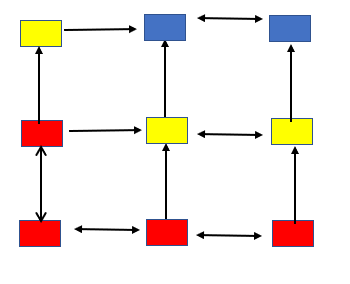
\includegraphics[scale=0.8]{grid.png}
\caption{The grid is a simplified gird showing how the discretised diffusion equation works in reality. A net heat flow is going from the warm grid points to those with a lower temperature, here visulised with red (warm), yellow (medium) and blue cold.\label{fig:tempgrid}}
\end{figure}
As one can see on the figure, it is possible to hold one of the positional variables constant while integrating the other. Thus the algorithms \ref{alg:FWE_1D} through \ref{alg:CN_1D} requires very little modification, as each the algorithms only has to be run twice, one in each direction. 

\subsection*{The Lithosphere}

Now that we have a system via which we may approximate the diffusion equation (and therefore the heat equation) numerically, we can apply these abstract concepts to a real-life scenario – the radioactive refertilization of the Fennoscandic\footnote{Fennoscandia refers to the Scandinavian peninsula, including Finland.} mantle.

More specifically, geologists theorize that there once existed a subduction zone in the Fennoscandic mantle.  An interesting consequence of such a subduction zone is that it would have lead to contact between the mantle and a vast number of ocean sediments\footnote{These may have contained a variety of relatively unstable elements, such as Uranium, Thorium, and Potassium.}.  As a result, the heat generation in the mantle is theorized to have increased due to the radioactive decay of these sediments.

To investigate this, we will be creating a more detailed model in which heat generation occurs over the entire simulated array, at rates defined by its depth.  We will be creating a model that represents a 150km deep, 200km wide 2-D slice of the lithosphere; we will divide this array into three depths: 

\begin{table}[H]
\center
\begin{tabular}{|c|ccc|}
\hline
Name & Upper Depth [km] & Lower Depth [km] & Heat Production [µW/m\textsuperscript{3}] \\
\hline
Upper Crust & 0 & 20 & 1.4 \\
Lower Crust & 20 & 40 & 0.35 \\
Mantle & 40 & 120 & 0.05 \\
\hline
\end{tabular}
\caption{The heat production for different sections of the lithosphere. \label{table_1}}
\end{table}

We will be using the heat equation presented in (\ref{eq_heat}), and as such we will set our thermal conductivity to $k = 2.5$W/m$^\circ$C, our density to $\rho = 3.5 \times 10^3$ kg/m\textsuperscript{3}, and our specific heat capacity to $c_p = 1000$J/kg$^\circ$C.

To simulate the radioactive refertilization of the mantle, we will also be adding a variable heat production to the mantle.  We will begin with an initial heat production of $Q_\text{rad,0} = 0.5$µW/m\textsuperscript{3}, but this will decline over time in a manner determined by the half-lives of the decaying particles.  To calculate this decline, we will be focusing on the decay of Uranium, Thorium, and Potassium, and assume the following:

\begin{table}[H]
\center
\begin{tabular}{|c|cc|}
\hline
Element & Half-Life [Gy] & Percent of Sediments \\
\hline
Uranium & 4.47 & 40\% \\
Thorium & 14.0 & 40\% \\
Potassium & 1.25 & 20\%\\
\hline
\end{tabular}
\caption{Distribution and half-lives of the most prominent radioactive sediments in the mantle. \label{table_2}}
\end{table}

Since the radioactive heat production decreases over time, we must create a function $Q_\text{rad}(t)$ using the above data.  To begin, we will need a general equation for \textit{exponential decay}:

\begin{equation*}
I(t) = I_0 \left( \frac{1}{2} \right)^{\tfrac{t}{t_{1/2}}}
\end{equation*}

Where $I(t)$ is the intensity of an exponentially decreasing process over time, $I_0$ is the initial intensity, $t$ is time, and $t_{1/2}$ is the half-life of the governing quantity.

We can apply these principles to a system of three decaying quantities, via the following:

\begin{equation*}
Q_\text{rad}(t) = Q_\text{rad,0} \left( 0.4 \left( \frac{1}{2} \right)^{\tfrac{t}{4.47 \times 10^9}} + 0.4 \left( \frac{1}{2} \right)^{\tfrac{t}{1.4 \times 10^{10}}} + 0.2 \left( \frac{1}{2} \right)^{\tfrac{t}{1.25 \times 10^9}} \right)
\end{equation*}

Finally, we can use all the information presented in this subsection, in conjunction with (\ref{eq_heat}), to give us the differential equation we will be solving:

\begin{boxquote}
\begin{equation}
\label{eq_lithosphere}
2.5 \nabla^2 T + Q_\text{tot}(t,y) =  3.5 \times 10^6 \frac{\partial T}{\partial t}
\end{equation}

With the total heat production $Q_\text{tot}$ given by two terms:

\begin{equation}
Q_\text{tot}(t,y) = Q(y) + Q_{rad}(t)
\end{equation}

Where the first term depends on the depth $y$:

\begin{equation}
Q(y) = \begin{cases} \mbox{1.4,} & \mbox{if } -20 < y < 0 \\ \mbox{0.35,} & \mbox{if } -40 \leq y < 20 \\ \mbox{0.05,} & \mbox{if } -120 \leq y < -40 \end{cases}
\end{equation}

And the second term is given by:

\begin{equation}
Q_\text{rad}(t) = 0.2 \left( \frac{1}{2} \right)^{\tfrac{t}{4.47 \times 10^9}} + 0.2 \left( \frac{1}{2} \right)^{\tfrac{t}{1.4 \times 10^{10}}} + 0.1 \left( \frac{1}{2} \right)^{\tfrac{t}{1.25 \times 10^9}}
\end{equation}
\end{boxquote}

This is unlikely to have a nice analytical solution, but if we omit the radioactive heat producing term, we can apply the methods presented in \textbf{Solving the Diffusion Equation} and \textbf{The Heat Equation} to find an analytical result.

\section*{Results}

We attempted to compare the analytical solution to the 1-D diffusion equation to the corresponding numerical results, and ended up with the following result for a 1-D row of zeros, appended by a single one.  The simulation ran for 0.1 dimensionless units of time, with $dt = 10^{-3}$; the row has a dimensionless length of 0.2, with $dx = 10^{-2}$.

\begin{figure}[H]
\centering
{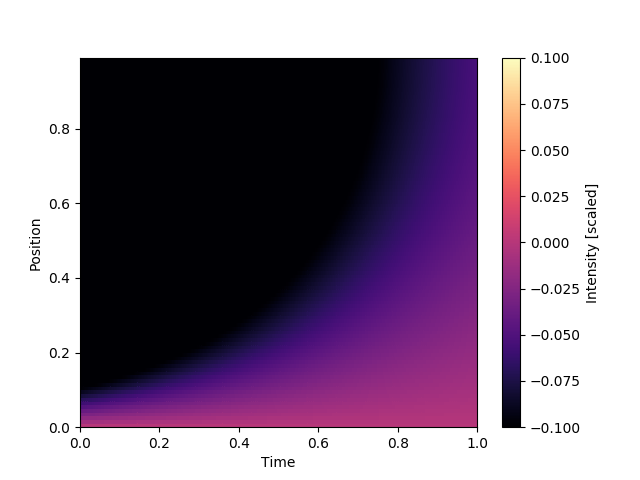
\includegraphics[width=0.8\textwidth]{analytical_solution.png}}
\caption{The analytical solution for the diffusion equation.\label{fig_0}}
\end{figure}

\begin{figure}[H]
 \centering
  {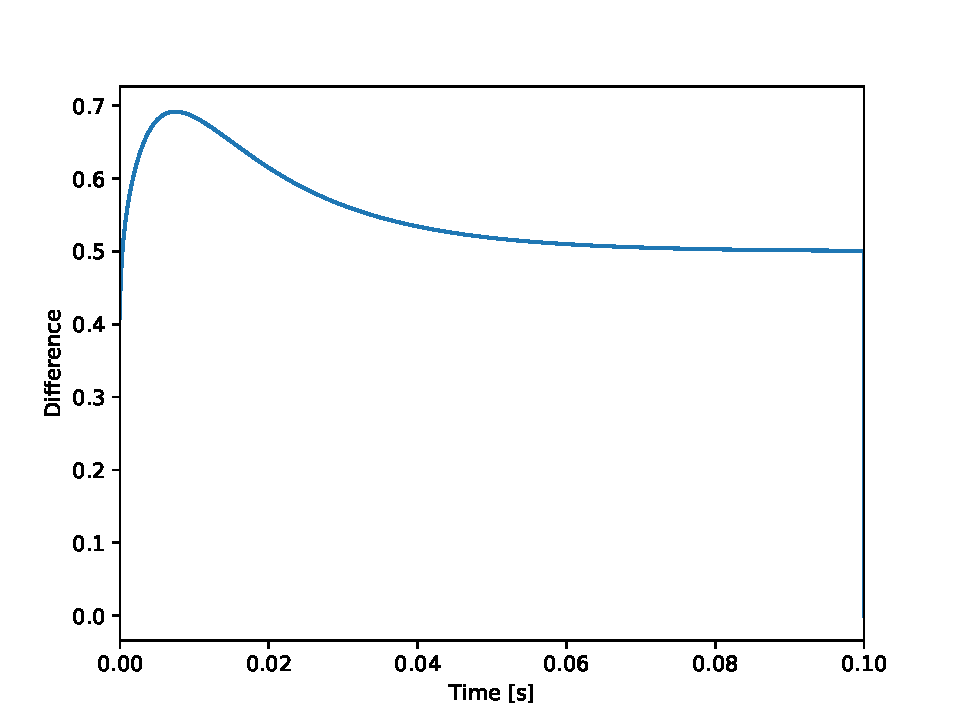
\includegraphics[width=0.8\textwidth]{fig1_fwd.pdf}}
  \caption{The mean difference in the 1-D numerical and analytical solution of the diffusion equation over time, using the \textit{Forward Euler} algorithm.\label{fig_5}}
\end{figure}

\begin{figure}[H]
 \centering
  {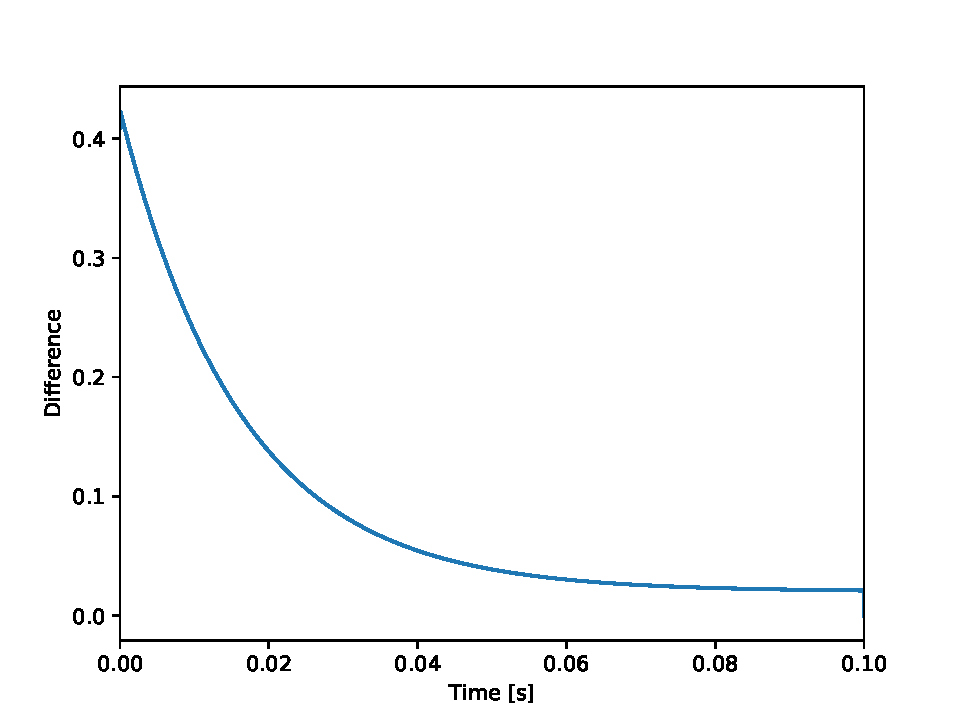
\includegraphics[width=0.8\textwidth]{fig1_bwd.pdf}}
  \caption{The mean difference in the 1-D numerical and analytical solution of the diffusion equation over time, using the \textit{Backward Euler} algorithm.\label{fig_6}}
\end{figure}

Using the same simulation settings, we then changed $dt$ such that the ratio $\frac{dt}{dx^2}$ would vary between 0.1 and 0.75, and ran each simulation for 50 different ratios and kept the mean difference in each final time step:

\begin{figure}[H]
 \centering
  {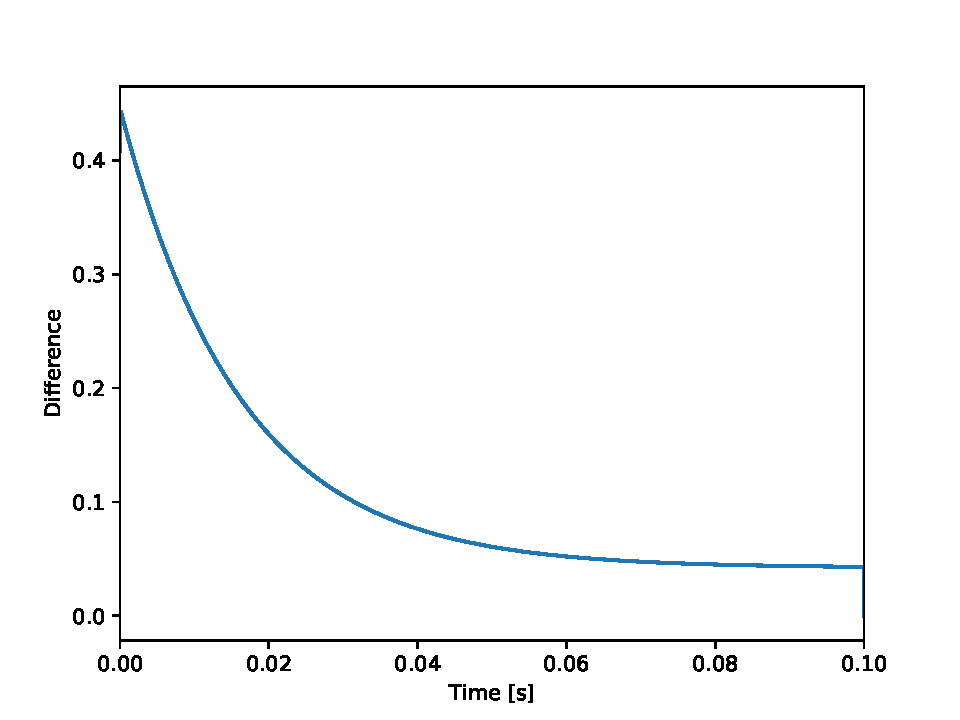
\includegraphics[width=0.8\textwidth]{fig1_crank.pdf}}
  \caption{The mean difference in the 1-D numerical and analytical solution of the diffusion equation over time, using the \textit{Crank-Nicolson} algorithm.\label{fig_7}}
\end{figure}

\begin{figure}[H]
 \centering
  {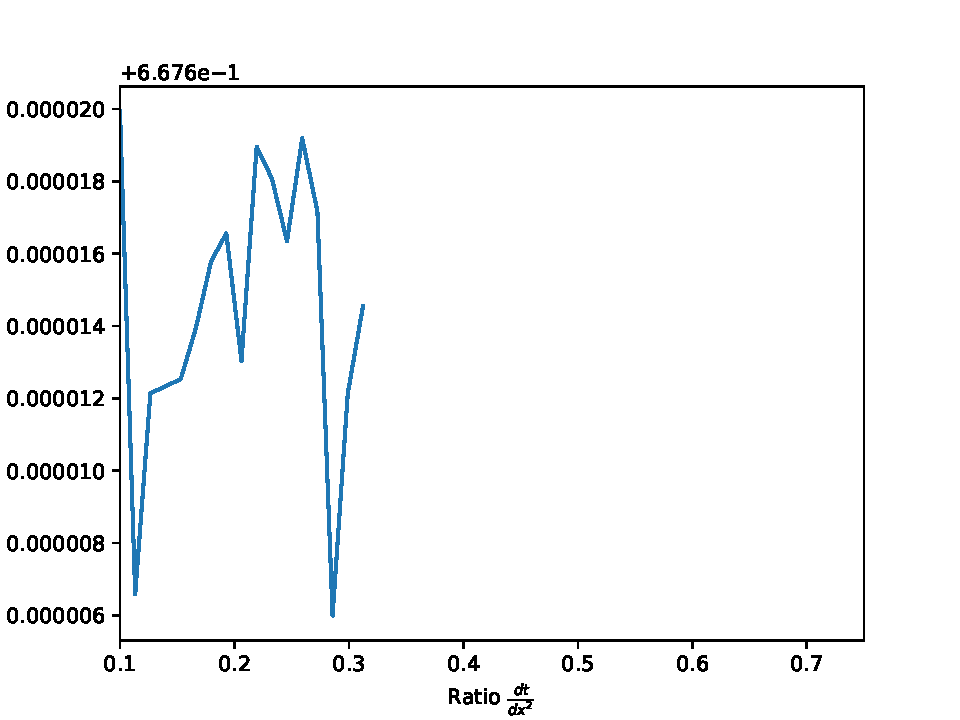
\includegraphics[width=0.8\textwidth]{fig2_fwd.pdf}}
  \caption{The mean difference in the 1-D numerical and analytical solution of the diffusion equation as a function of the ratio $\frac{dt}{dx^2}$, using the \textit{Forward Euler} algorithm.\label{fig_8}}
\end{figure}

\begin{figure}[H]
 \centering
  {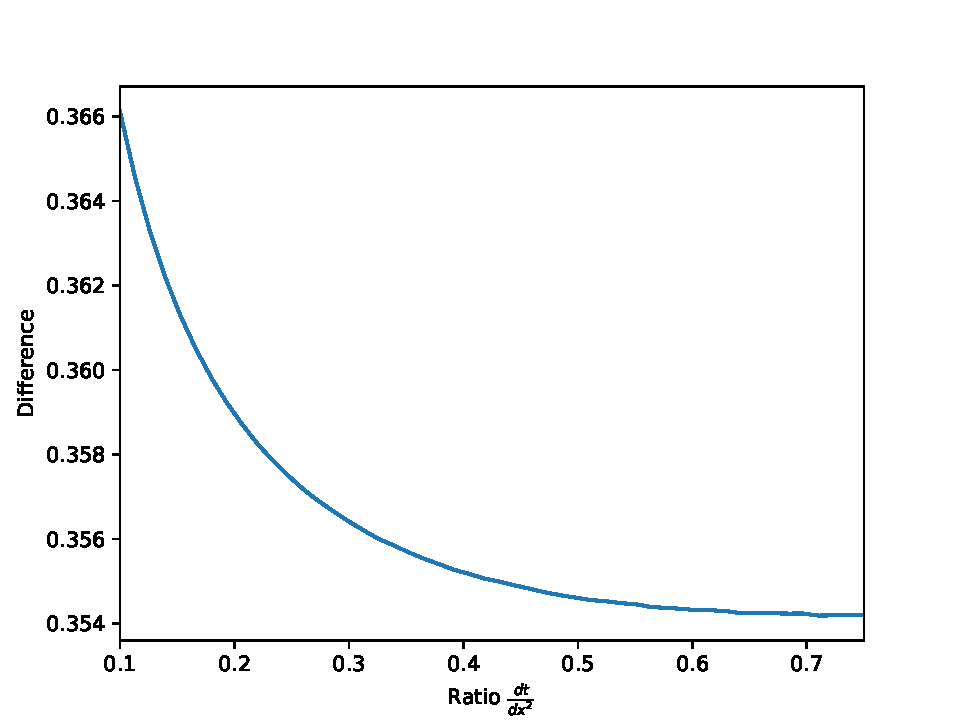
\includegraphics[width=0.8\textwidth]{fig2_bwd.pdf}}
  \caption{The mean difference in the 1-D numerical and analytical solution of the diffusion equation as a function of the ratio $\frac{dt}{dx^2}$, using the \textit{Backward Euler} algorithm.\label{fig_9}}
\end{figure}

\begin{figure}[H]
 \centering
  {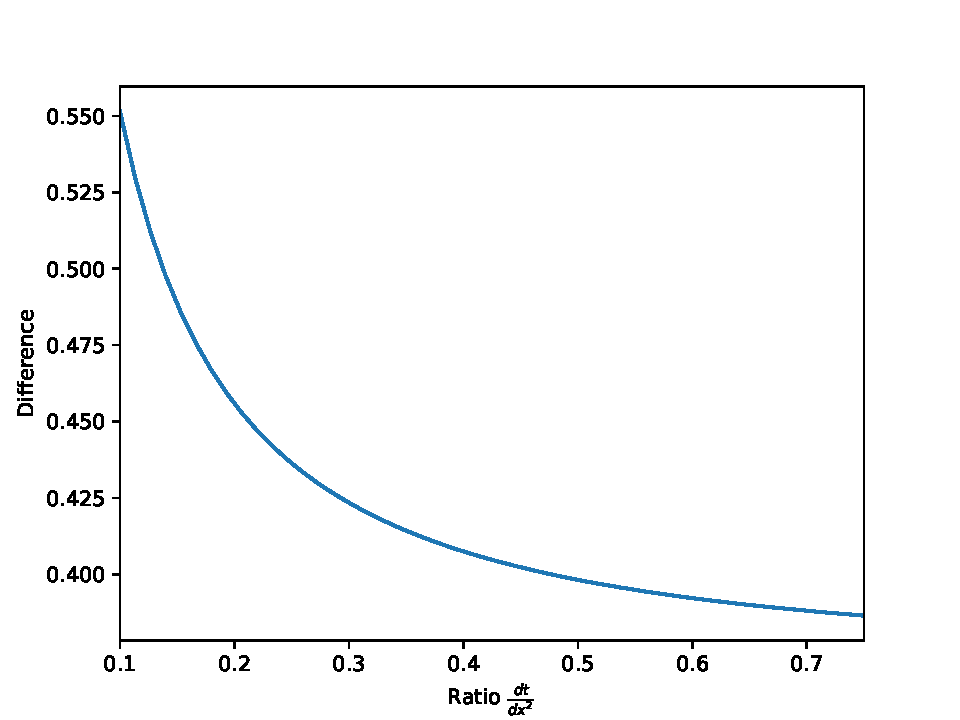
\includegraphics[width=0.8\textwidth]{fig2_cra.pdf}}
  \caption{The mean difference in the 1-D numerical and analytical solution of the diffusion equation as a function of the ratio $\frac{dt}{dx^2}$, using the \textit{Crank-Nicolson} algorithm.\label{fig_10}}
\end{figure}

Next, we implemented the algorithms presented in \ref{alg:FWE_1D}, \ref{alg:BWE_1D}, and \ref{alg:CN_1D} on a simple set of initial conditions, whereby we have a grid of zeros whose right side is composed of ones.  Each simulation ran for $100$ dimensionless units of time, with a time step of $dt = 10^{-3}$; each grid has a height and width of $40 \times 10$, with $dx = 1$.

\begin{figure}[H]
 \centering
    \subfloat[]{{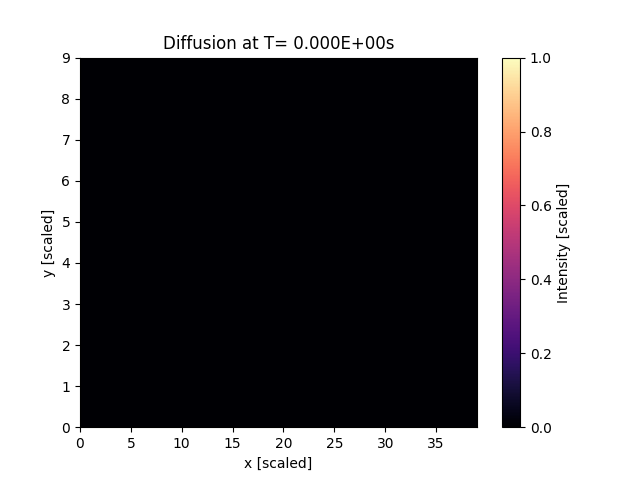
\includegraphics[width=.5\textwidth]{fwd_0.png} }}
    \subfloat[]{{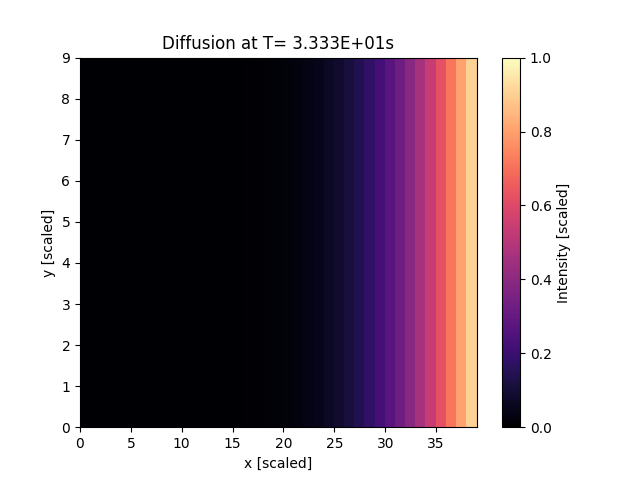
\includegraphics[width=.5\textwidth]{fwd_1.png} }}
   	    \qquad
    \subfloat[]{{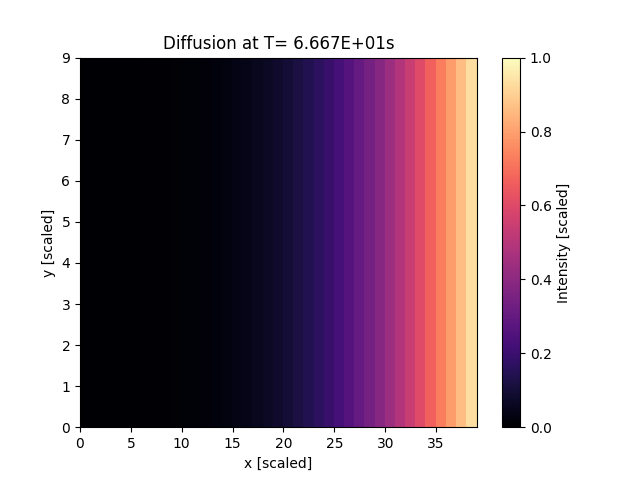
\includegraphics[width=.5\textwidth]{fwd_2.png} }}
    \subfloat[]{{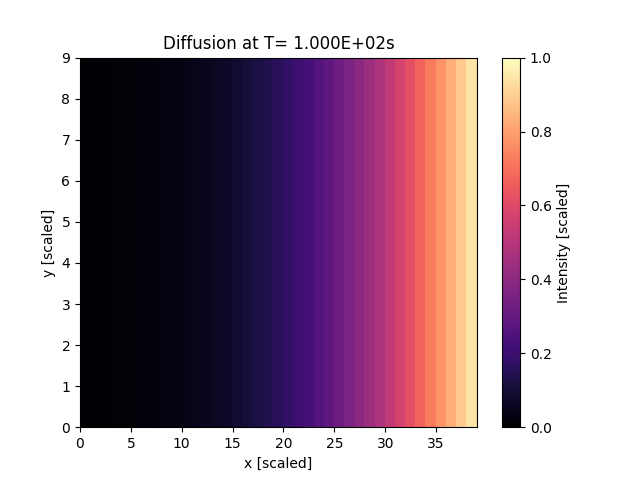
\includegraphics[width=.5\textwidth]{fwd_3.png} }}
    \caption{The 2-D diffusion equation using the \textit{Forward Euler} algorithm.\label{fig_1}}
\end{figure}

\begin{figure}[H]
 \centering
    \subfloat[]{{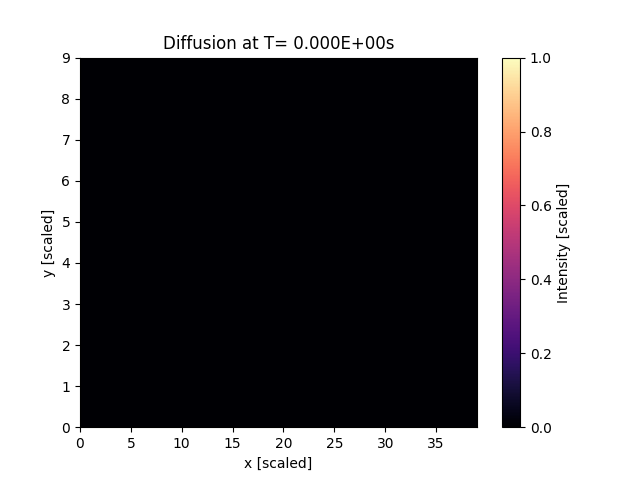
\includegraphics[width=.5\textwidth]{bwd_0.png} }}
    \subfloat[]{{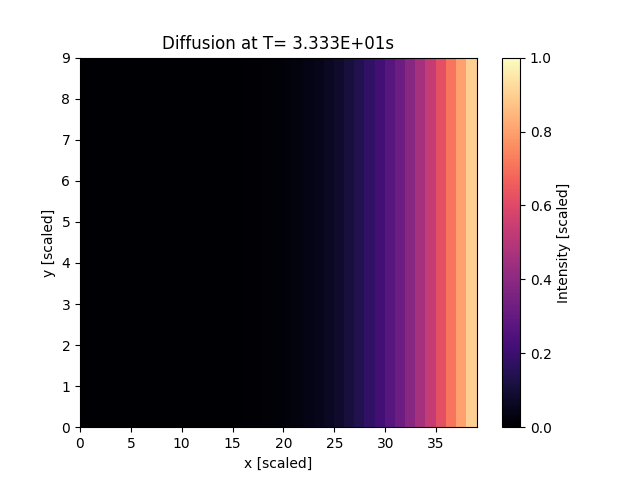
\includegraphics[width=.5\textwidth]{bwd_1.png} }}
   	    \qquad
    \subfloat[]{{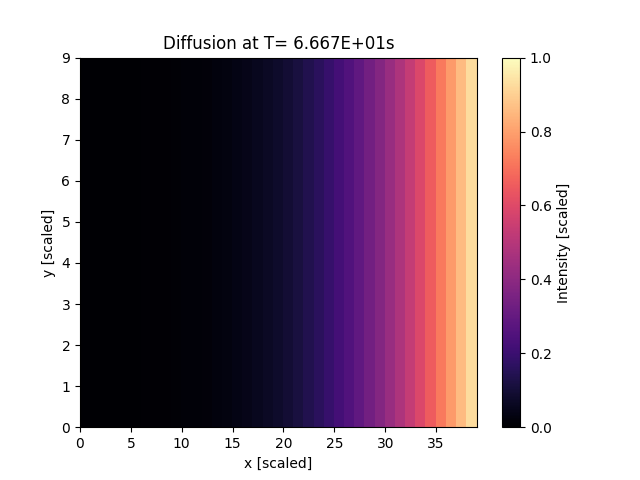
\includegraphics[width=.5\textwidth]{bwd_2.png} }}
    \subfloat[]{{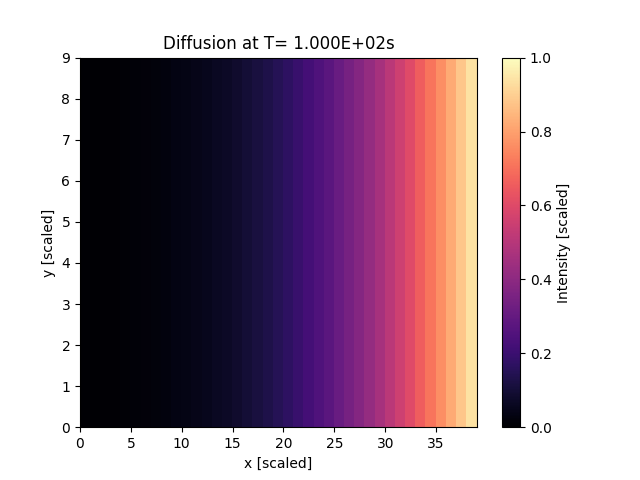
\includegraphics[width=.5\textwidth]{bwd_3.png} }}
    \caption{The 2-D diffusion equation using the \textit{Backward Euler} algorithm.\label{fig_2}}
\end{figure}

\begin{figure}[H]
 \centering
    \subfloat[]{{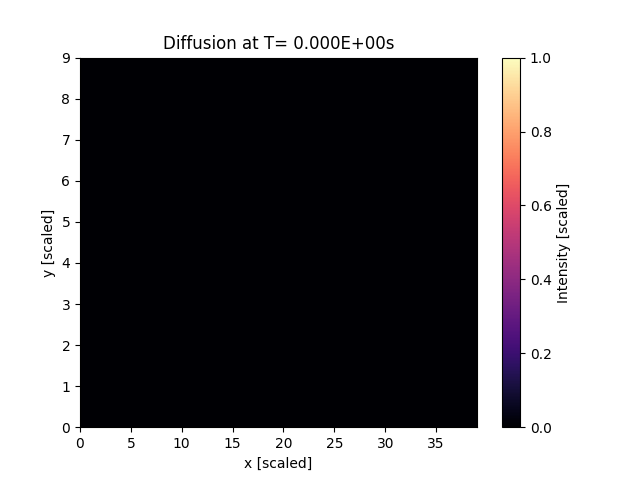
\includegraphics[width=.5\textwidth]{cra_0.png} }}
    \subfloat[]{{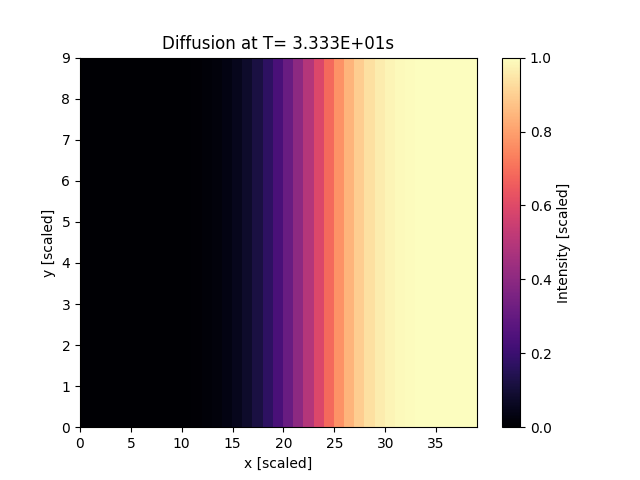
\includegraphics[width=.5\textwidth]{cra_1.png} }}
   	    \qquad
    \subfloat[]{{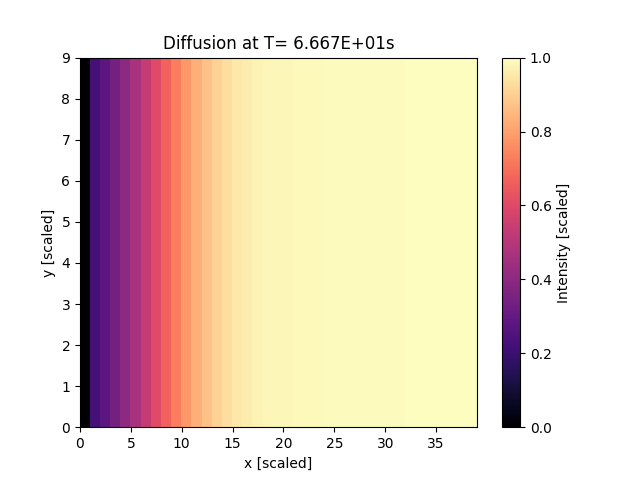
\includegraphics[width=.5\textwidth]{cra_2.png} }}
    \subfloat[]{{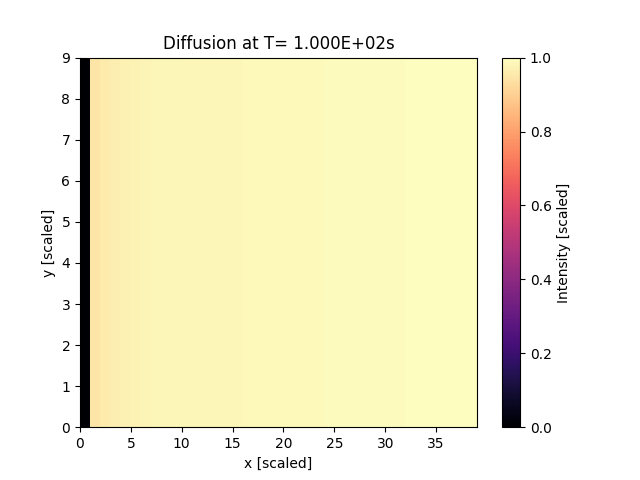
\includegraphics[width=.5\textwidth]{cra_3.png} }}
    \caption{The 2-D diffusion equation using the \textit{Crank Nicolson} algorithm.\label{fig_3}}
\end{figure}

Using the 2-D Forward Euler algorithm, we modeled the Fennoscandian lithosphere over the course of one-billion years, and over an area 150km deep and 150km wide.  We used a time step of $dt = 5 \times 10^6$ years, with $dx = 10^3$ km.

\begin{figure}[H]
 \centering
    \subfloat[]{{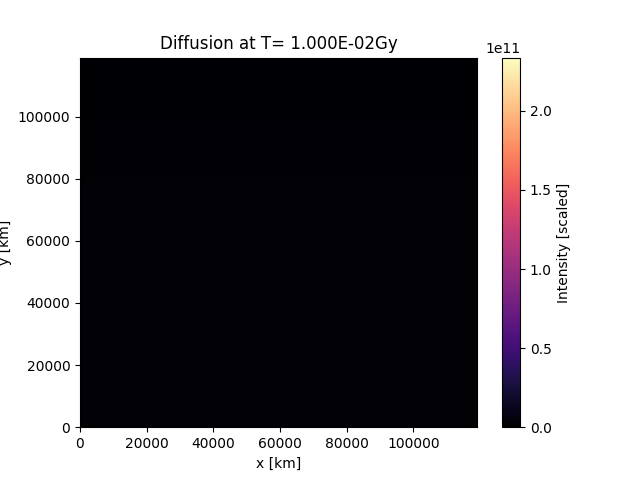
\includegraphics[width=.5\textwidth]{fwd_litho_0.png} }}
    \subfloat[]{{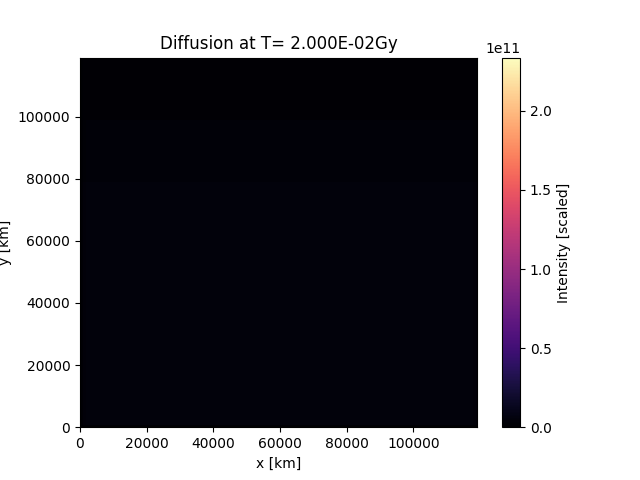
\includegraphics[width=.5\textwidth]{fwd_litho_1.png} }}
   	    \qquad
    \subfloat[]{{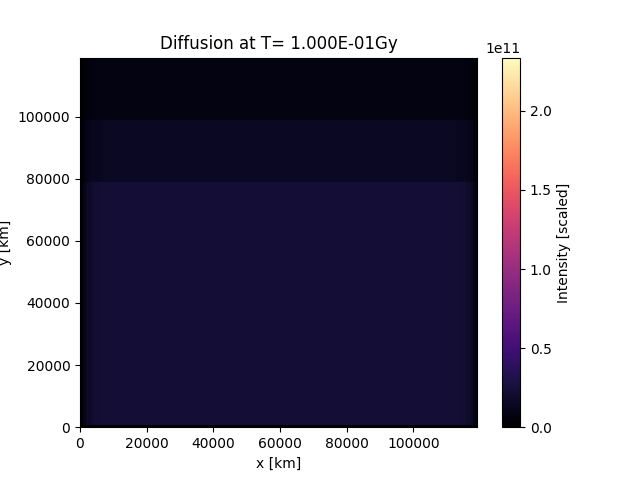
\includegraphics[width=.5\textwidth]{fwd_litho_2.png} }}
    \subfloat[]{{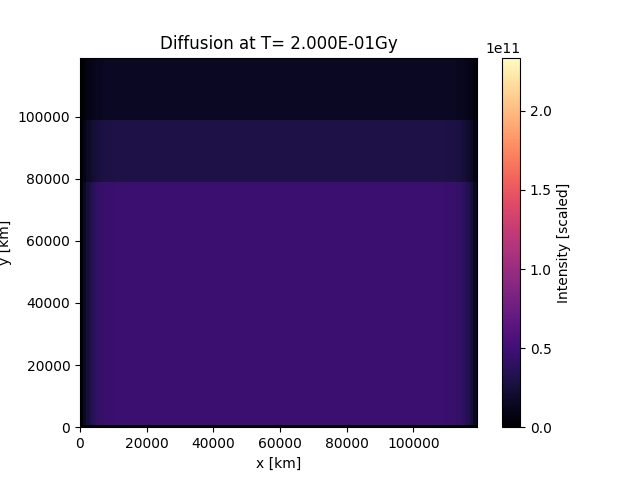
\includegraphics[width=.5\textwidth]{fwd_litho_3.png} }}
   	    \qquad
    \subfloat[]{{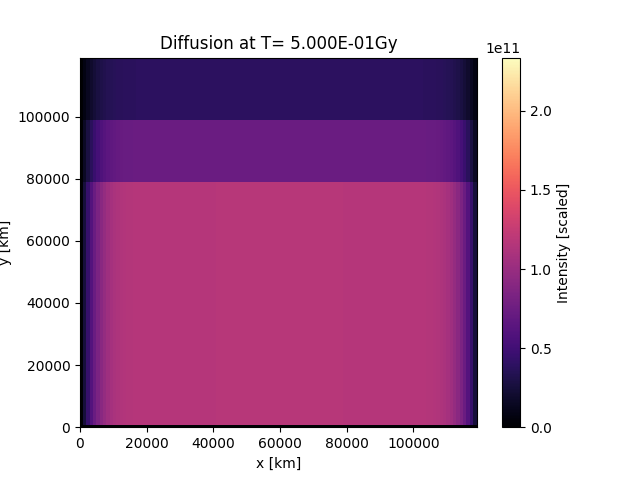
\includegraphics[width=.5\textwidth]{fwd_litho_4.png} }}
    \subfloat[]{{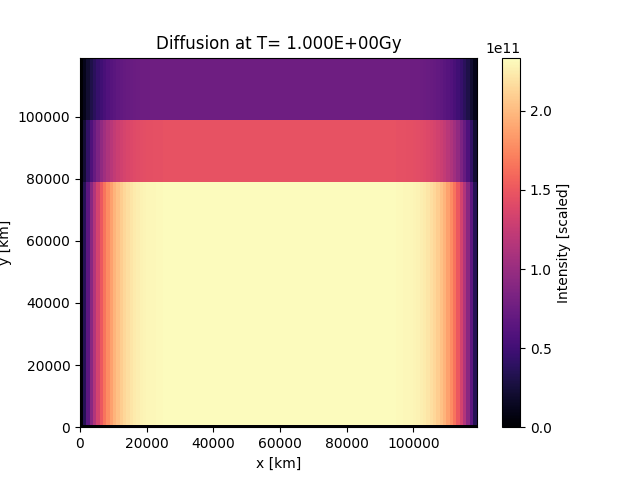
\includegraphics[width=.5\textwidth]{fwd_litho_5.png} }}
    \caption{The 2-D diffusion equation modeling the lithosphere model presented in \textbf{The Lithosphere}, using the \textit{Forward Euler} algorithm.\label{fig_4}}
\end{figure}

\section*{Discussion}

\subsection*{The 1-D Diffusion Equation}

We begin with the analytical solution shown in Figure \ref{fig_0}, whose time-position distribution matches our expectation that the heat will spread at a rate governed by equation (\ref{eq_analytical}).

Using this, we then have Figures \ref{fig_5}, \ref{fig_6}, and \ref{fig_7} which show the mean differences between the Forward Euler, Backward Euler, and Crank-Nicolson algorithms and the analytical solution as a function of time, which show that the model is more precise as time passes, rather then initially precise and less precise over time.

To determine how to best set up our ratio $\frac{dt}{dx^2}$, we see in Figure \ref{fig_8} that the Forward Euler algorithm breaks down when $\frac{dt}{dx^2} > 0.4$, and that the difference between the analytical and numerical solutions are minimized near this point.  

The Backward Euler algorithm shown in Figure \ref{fig_9} is not restricted in such a way, nor is its analytical-numerical difference minimized at the aforementioned ratio, but the model doesn't break down once the ratio increases past that point and simply becomes more precise as the ratio increases.

As for the Crank-Nicolson algorithm shown in Figure \ref{fig_10}, we see that the ratio gets continuously better as it increases, mirroring much of the behavior of the Backward Euler algorithm.


It is important to note that the backward Euler algorithm, as we implemented it, seems to be slightly better than the Crank-Nicolson scheme. Considering the fact that Crank-Nicolson is a higher degree numerical scheme, with an error of $O(\Delta t^2)$ while Backward Euler is a first order method, as explained in \cite{compendium}. This becomes especially clear if we compare the figures \ref{fig_9} and \ref{fig_10}, where while their performance is similar, the Backwards Euler scheme does slightly better. If one then looks at figures \ref{fig_3} one can see the temperature in the system rapidly does increase, which doesn't happen at all in the backward Euler case. 
\subsection*{The 2-D Diffusion Equation}

Our results in Figures \ref{fig_1} and \ref{fig_2} appear to match quite well, these being the Forward and Backward Euler alogorithm results.  As expected, the heat spreads from the right to left and dissipates as a function of distance, in a nearly identical way.  This implies that our results are likely correct, as these algorithms differ rather significantly in their implementations.

On the other hand, the Crank-Nicolson algorithm results shown in Figure \ref{fig_3} don't appear to give the same results as our two other algorithms.  Here, the heat spreads much more intensely as we move away from the section adjacent to the right boundary, when compared to Figures \ref{fig_1} and \ref{fig_2}.

\subsection*{The Lithosphere}

In our lithosphere model, we investigated the heat distribution in the mantle and crust over a billion years; given the results shown in Figure \ref{fig_4}, we found that these generally matched our expectations – the heat was most concentrated in the mantle and slowly spread upwards toward the lower and upper crusts.  In addition to this, we noticed that the temperature in the mantle tended to increase over time without stopping, likely due to the fact that the radioactive decay had not yet decreased by a significant enough amount at that point in time.

\section*{Conclusion}

Overall, it appears as though our numerical models are imperfect when compared to their analytical counterpart, yet we can still see that the general trend and rates of diffusion remain proportional to those found in the analytical solutions – this suggests that there may be a scaling issue with our algorithms that managed to get by unnoticed.  Nevertheless, we can conclude that our numerical approximations are close enough to be used with confidence in our lithospheric model, as the differences in our 1-D analytical and numerical solutions are not so large as to merit the discounting of our models.


We also have reason to believe that the Crank-Nicolson scheme was implemented incorrectly, as the diffusion is extremely rapid and ends up dominating the entire system. Our most likely guess for this is that the lower boundary condition $u(0,t)=0$ wasn't correctly implemented in the algorithm, but due to time constraints we did not manage to fix this problem. 


Having concluded that our model is close enough, we then carried on our lithosphere simulation, and observed that the temperature in the mantle increased significantly over the course of a billion years; this makes sense, as the radioactive heat production in the mantle did not decrease by a noticeable amount over the course of the simulation, as the shortest half-life was longer than the simulation runtime.

Unfortunately, we cannot conclude with certainty as to whether or not our lithosphere model follows the true course of the Fennoscandian geological evolution, however it is somewhat unlikely that the temperature would increase so much over the last billion years without consequence to the surrounding environment, so there is most likely a number of factors being left our of this simulation that would more accurately reflects reality.

\bibliography{bib}{}
\bibliographystyle{IEEEtran}
\end{document}
